\documentclass{beamer}
%\documentclass[handout]{beamer}

% language settings
%\usepackage{fontspec, polyglossia}
%\setdefaultlanguage{magyar}

% common packages
%\usepackage{amsmath, multimedia, hyperref, multirow}
\usepackage{amsmath, multimedia, hyperref, xcolor, multirow}
%\usepackage{graphicx}

% TikZ
\usepackage{tikz}
\usetikzlibrary{arrows.meta, decorations.pathmorphing, decorations.pathreplacing, shapes.geometric,mindmap}
%\usetikzlibrary{shapes.geometric,fadings,bayesnet}

% beamer styles
\mode<presentation>{
\usetheme{Singapore}
%\usetheme{Pittsburgh}
\usecolortheme{orchid}
%\usecolortheme{seahorse}
%\usefonttheme{structureitalicserif}
\setbeamercovered{transparent}
}
\setbeamertemplate{blocks}[rounded][shadow=true]
%\AtBeginSubsection[]{
%  \begin{frame}<beamer>{Contents}
%    \tableofcontents[currentsection,currentsubsection]
%  \end{frame}
%}
%\useoutertheme[]{tree}

% title, etc
\title{Probabilistic Combination and Filtering of Callers}
\subtitle{Benchmark Experiment and Machine Learning}
\author{Attila Gulyas-Kovacs, Chaggai Rosenbluh, Andy Chess}
\date{Chess Lab, Mount Sinai}

\begin{document}

\maketitle

\section{Introduction}

\begin{frame}{Schizophrenia genetics}

\includegraphics<1>[width=1.0\textwidth]{figures/from-others/ripke2014nature-fig1.png}

\only<1>{\tiny Ripke et al Nature.~2014}

\includegraphics<2>[width=0.7\textwidth]{figures/from-others/ripke2013natgen-fig1a.jpg}
\only<2>{\tiny Ripke et al Nat Genet.~2013}
\end{frame}

\begin{frame}{Our workflow}
\footnotesize
\begin{enumerate}
\item
\begin{itemize}
\item
brain sample \tikz[baseline=-0.5ex] \draw[->] (0,0) -- node[above] (A)
{NeuN+, PCR-free, HiSeq, align} (4.5,0); \texttt{neuron.bam}
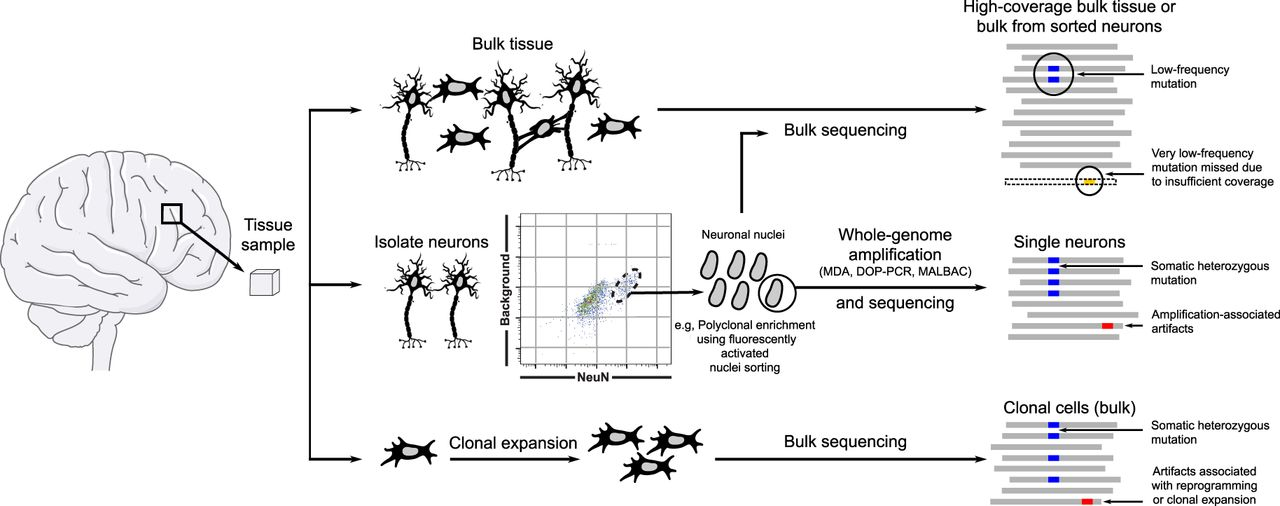
\includegraphics[width=0.7\textwidth]{figures/bsm-science-fig2.jpg}
\item<2->
muscle sample \tikz[baseline=-0.5ex] \draw[->] (0,0) -- node[above] (A)
{PCR-free, HiSeq, align} (4.5,0); \texttt{muscle.bam}
\end{itemize}
\item<3->
\begin{itemize}
\item \texttt{TNseq.Mutect2.vcf}
\item \texttt{lofreqSomatic.vcf}
\item \texttt{somaticSniper.vcf}
\item \texttt{strelka2Germline2s.vcf}
\item \texttt{strelka2Somatic.vcf}
\end{itemize}
\item<4-> \tikz[baseline=-0.5ex] \draw[->] (0,0) -- node[above] (A)
{machine learning} (2.5,0); \texttt{VariantMetaCaller.vcf}
\begin{itemize}
\item probabilistic combination and filtering
\end{itemize}
\end{enumerate}
\end{frame}

\begin{frame}
\includegraphics[height=0.9\textheight]{figures/2018-11-06-number-of-calls/snvs-1.pdf}
\end{frame}

\begin{frame}<1>[label=hardfilterlimit]{Limitations of traditional filtering}
\begin{enumerate}
\item<1-> unknown precision \(\Rightarrow\) callers not comparable
\begin{itemize}
\item<3-> labeled benchmark data: true precision \& recall
\item<4-> machine learning: estimated precision
\end{itemize}
\item<2-> discards info in the interdependence of annotations
\begin{itemize}
\item<4-> machine learning
\end{itemize}
\end{enumerate}
\end{frame}

\begin{frame}{Controlling precision}
\[\mathrm{precision} = 1 - \mathrm{FDR}\]
\begin{columns}[t]
\begin{column}{0.5\textwidth}
\begin{center}
without control
\end{center}
\includegraphics<1-2>[width=1\columnwidth]{figures/by-me/precision-recall/pr-realistic.pdf}
\end{column}

\begin{column}{0.5\textwidth}
\begin{center}
\only<2>{with control }
\end{center}
\includegraphics<2>[width=1\columnwidth]{figures/by-me/precision-recall/pr.pdf}
\end{column}
\end{columns}
\end{frame}

\againframe<2>{hardfilterlimit}

\begin{frame}
\textbf{unfiltered VCF}

\tikz[baseline=-0.5ex] \path (0,0) -- node[draw, fill=red, rectangle, inner
sep=3.0pt] {} (1,0);true positive

\tikz[baseline=-0.5ex] \path (0,0) -- node[draw, fill=blue, circle, inner
sep=2.5pt] {} (1,0);false positive
\begin{columns}[t]
\begin{column}{0.5\textwidth}
\begin{center}
\only<1>{calls}
\only<2->{traditional filtering}
\end{center}

\includegraphics<1>[width=1\columnwidth]{figures/by-me/vcf-annot-classif/strelka2/strelka2.pdf}

\includegraphics<2->[width=1\columnwidth]{figures/by-me/vcf-annot-classif/strelka2/strelka2-hardfilter.pdf}
\end{column}

\begin{column}{0.5\textwidth}
\begin{center}
\only<3>{flexible filtering}
\end{center}

\includegraphics<3>[width=1\columnwidth]{figures/by-me/vcf-annot-classif/strelka2/strelka2-svm.pdf}
\end{column}
\end{columns}
\end{frame}

\againframe<4->{hardfilterlimit}

\section{Benchmark}

\begin{frame}{Benchmark experiment}
\begin{center}
labeled callset \(j\): \(\{\overbrace{y_{ij}}^\text{label},
\overbrace{\mathbf{x}_{ij}}^\text{annot}\}_{i=1,...,n_j}\)
\end{center}
\vfill

\tiny
\setlength{\tabcolsep}{3pt}
\begin{tabular}{|l|llllllll|}
\hline
\footnotesize label &
\multicolumn{8}{|c|}{\footnotesize annotations: \texttt{TNseq.Mutect2.vcf}} \\
\hline
\(y_{\cdot,1}\) & \#CHROM & POS & ID & REF & ALT & QUAL & FILTER & INFO \\
\textcolor{black}{0} &
\textcolor{black}{1} &
\textcolor{black}{50003788} &
\textcolor{black}{0} &
\textcolor{black}{A} &
\textcolor{black}{G} &
\textcolor{black}{0} &
\textcolor{black}{t\_lod\_fstar} &
\textcolor{black}{...;NLOD=30.4;TLOD=4.62} \\
\bfseries \textcolor{black}{1} &
\bfseries \textcolor{black}{1} &
\bfseries \textcolor{black}{50005034} &
\bfseries \textcolor{black}{0} &
\bfseries \textcolor{black}{G} &
\bfseries \textcolor{black}{T} &
\bfseries \textcolor{black}{0} &
\bfseries \textcolor{black}{t\_lod\_fstar} &
\bfseries \textcolor{black}{...;NLOD=33.27;TLOD=4.51} \\
\bfseries \textcolor{black}{1} &
\bfseries \textcolor{black}{1} &
\bfseries \textcolor{black}{50007349} &
\bfseries \textcolor{black}{0} &
\bfseries \textcolor{black}{C} &
\bfseries \textcolor{black}{T} &
\bfseries \textcolor{black}{0} &
\bfseries \textcolor{black}{PASS} &
\bfseries \textcolor{black}{...;NLOD=23.43;TLOD=10.97} \\
\textcolor{black}{0} &
\textcolor{black}{1} &
\textcolor{black}{50008565} &
\textcolor{black}{0} &
\textcolor{black}{C} &
\textcolor{black}{A} &
\textcolor{black}{0} &
\textcolor{black}{PASS} &
\textcolor{black}{...;NLOD=7.69;TLOD=8.26} \\
\hline
% \vdots & \vdots & \vdots & \vdots & \vdots & \vdots & \vdots & \vdots & \vdots & \vdots & \vdots \\
\end{tabular}
\tiny
\\[1em]
\begin{tabular}{|l|llllllll|}
\hline
\footnotesize label &
\multicolumn{8}{|c|}{\footnotesize annotations: \texttt{strelka2Somatic.vcf}} \\
\hline
\(y_{\cdot,2}\) & \#CHROM & POS & ID & REF & ALT & QUAL & FILTER & INFO \\
\bfseries \textcolor{black}{1} &
\bfseries \textcolor{black}{1} &
\bfseries \textcolor{black}{50003323} &
\bfseries \textcolor{black}{0} &
\bfseries \textcolor{black}{A} &
\bfseries \textcolor{black}{G} &
\bfseries \textcolor{black}{0} &
\bfseries \textcolor{black}{LowEVS} &
\bfseries \textcolor{black}{...;DP=274;MQ=59.86;...;SomaticEVS=0} \\
\textcolor{black}{0} &
\textcolor{black}{1} &
\textcolor{black}{50003455} &
\textcolor{black}{0} &
\textcolor{black}{C} &
\textcolor{black}{T} &
\textcolor{black}{0} &
\textcolor{black}{LowEVS} &
\bfseries \textcolor{black}{...;DP=226;MQ=59.9;...;SomaticEVS=0.65} \\
\bfseries \textcolor{black}{1} &
\bfseries \textcolor{black}{1} &
\bfseries \textcolor{black}{50005034} &
\bfseries \textcolor{black}{0} &
\bfseries \textcolor{black}{G} &
\bfseries \textcolor{black}{T} &
\bfseries \textcolor{black}{0} &
\bfseries \textcolor{black}{PASS} &
\bfseries \textcolor{black}{...;DP=278;MQ=59.95;...;SomaticEVS=9.04} \\
\bfseries \textcolor{black}{1} &
\bfseries \textcolor{black}{1} &
\bfseries \textcolor{black}{50007349} &
\bfseries \textcolor{black}{0} &
\bfseries \textcolor{black}{C} &
\bfseries \textcolor{black}{T} &
\bfseries \textcolor{black}{0} &
\bfseries \textcolor{black}{LowEVS} &
\bfseries \textcolor{black}{...;DP=192;MQ=59.88;...;SomaticEVS=4.19} \\
\hline
% \vdots & \vdots & \vdots & \vdots & \vdots & \vdots & \vdots & \vdots & \vdots & \vdots & \vdots \\
\end{tabular}
% ##INFO=<ID=SomaticEVS,Number=1,Type=Float,Description="Somatic Empirical
% Variant Score (EVS) expressing the phred-scaled probability of thecall being
% a false positive observation.">
\normalsize

\end{frame}

\begin{frame}[label=benchmark]{Benchmark sample}{CEPH/Utah grandparents mixed}
\begin{center}
\begin{columns}[t]
\begin{column}{0.5\textwidth}

\includegraphics[width=1\textwidth]{figures/from-others/ceph-utah-pedigree-1463.png}
\end{column}

\begin{column}{0.5\textwidth}

\small
{\onslide<1->
\begin{tabular}{cccc}
genome & mix1 & mix2 & mix3\\
\hline
NA12889 & 4 & 2 & 0\\
NA12891 & 8 & 4 & 0\\
NA12890 & 16 & 8 & 0\\
NA12892 & 72 & 86 & 100\\
\hline
total & 100 & 100 & 100\\
\end{tabular}
}
\vfill
{\onslide<2->
\begin{tabular}{cc}
case:control & utility \\
\hline
\hline
mix1:mix3 & later somatic mut. \\
mix2:mix3 & later somatic mut. \\
\hline
mix1:mix1 & early somatic mut. \\
mix2:mix2 & early somatic mut. \\
\hline
mix3:mix3 & false calls \\
\end{tabular}
}
\end{column}
\end{columns}
\end{center}
\end{frame}

\begin{frame}{Impact of alternative allele frequency}
\includegraphics[width=1\textwidth]{figures/from-others/chaggai-recall-aaf.png}
\end{frame}

\begin{frame}[label=precrecall]{Callers in precision-recall space}
\includegraphics[width=1\textwidth]{figures/from-others/chaggai-precision-recall.png}
\end{frame}

\section{Machine Learning}

\begin{frame}{Machine learning}{VariantMetaCaller; Gezsi et al 2015 BMC Genomics}
%\begin{enumerate}
%\item annotation selection
%\begin{itemize}
%\item evaluate performance using benchmark; repeat
%\end{itemize}
%\item training SVMs
%\begin{itemize}
%\end{itemize}
%\item prediction  
%\begin{itemize}
%\item probabilistic filtering (precision/FDR)
%\item optimal combination of callsets
%\end{itemize}
%\end{enumerate}
\includegraphics[width=0.8\textwidth]{figures/from-others/vmc-fig1.png}
\end{frame}

\begin{frame}
\tiny
\setlength{\tabcolsep}{3pt}
\begin{tabular}{|l|llllllll|}
\hline
\footnotesize label &
\multicolumn{8}{|c|}{\footnotesize annotations: \texttt{TNseq.Mutect2.vcf}} \\
\hline
\(y_{\cdot,1}\) & \#CHROM & POS & ID & REF & ALT & QUAL & FILTER & INFO \\
\textcolor{cyan}{0} &
\textcolor{cyan}{1} &
\textcolor{cyan}{50003788} &
\textcolor{cyan}{0} &
\textcolor{cyan}{A} &
\textcolor{cyan}{G} &
\textcolor{cyan}{0} &
\textcolor{cyan}{t\_lod\_fstar} &
\textcolor{cyan}{...;NLOD=30.4;TLOD=4.62} \\
\bfseries \textcolor{cyan!50!brown}{1} &
\bfseries \textcolor{cyan!50!brown}{1} &
\bfseries \textcolor{cyan!50!brown}{50005034} &
\bfseries \textcolor{cyan!50!brown}{0} &
\bfseries \textcolor{cyan!50!brown}{G} &
\bfseries \textcolor{cyan!50!brown}{T} &
\bfseries \textcolor{cyan!50!brown}{0} &
\bfseries \textcolor{cyan!50!brown}{t\_lod\_fstar} &
\bfseries \textcolor{cyan!50!brown}{...;NLOD=33.27;TLOD=4.51} \\
\bfseries \textcolor{cyan!50!brown}{1} &
\bfseries \textcolor{cyan!50!brown}{1} &
\bfseries \textcolor{cyan!50!brown}{50007349} &
\bfseries \textcolor{cyan!50!brown}{0} &
\bfseries \textcolor{cyan!50!brown}{C} &
\bfseries \textcolor{cyan!50!brown}{T} &
\bfseries \textcolor{cyan!50!brown}{0} &
\bfseries \textcolor{cyan!50!brown}{PASS} &
\bfseries \textcolor{cyan!50!brown}{...;NLOD=23.43;TLOD=10.97} \\
\textcolor{cyan!50!brown}{0} &
\textcolor{cyan}{1} &
\textcolor{cyan}{50008565} &
\textcolor{cyan}{0} &
\textcolor{cyan}{C} &
\textcolor{cyan}{A} &
\textcolor{cyan}{0} &
\textcolor{cyan}{PASS} &
\textcolor{cyan}{...;NLOD=7.69;TLOD=8.26} \\
\hline
% \vdots & \vdots & \vdots & \vdots & \vdots & \vdots & \vdots & \vdots & \vdots & \vdots & \vdots \\
\end{tabular}
\tiny
\\[1em]
\begin{tabular}{|l|llllllll|}
\hline
\footnotesize label &
\multicolumn{8}{|c|}{\footnotesize annotations: \texttt{strelka2Somatic.vcf}} \\
\hline
\(y_{\cdot,2}\) & \#CHROM & POS & ID & REF & ALT & QUAL & FILTER & INFO \\
\bfseries \textcolor{brown}{1} &
\bfseries \textcolor{brown}{1} &
\bfseries \textcolor{brown}{50003323} &
\bfseries \textcolor{brown}{0} &
\bfseries \textcolor{brown}{A} &
\bfseries \textcolor{brown}{G} &
\bfseries \textcolor{brown}{0} &
\bfseries \textcolor{brown}{LowEVS} &
\bfseries \textcolor{brown}{...;DP=274;MQ=59.86;...;SomaticEVS=0} \\
\textcolor{brown}{0} &
\textcolor{brown}{1} &
\textcolor{brown}{50003455} &
\textcolor{brown}{0} &
\textcolor{brown}{C} &
\textcolor{brown}{T} &
\textcolor{brown}{0} &
\textcolor{brown}{LowEVS} &
\bfseries \textcolor{brown}{...;DP=226;MQ=59.9;...;SomaticEVS=0.65} \\
\bfseries \textcolor{brown}{1} &
\bfseries \textcolor{cyan!50!brown}{1} &
\bfseries \textcolor{cyan!50!brown}{50005034} &
\bfseries \textcolor{cyan!50!brown}{0} &
\bfseries \textcolor{cyan!50!brown}{G} &
\bfseries \textcolor{cyan!50!brown}{T} &
\bfseries \textcolor{cyan!50!brown}{0} &
\bfseries \textcolor{cyan!50!brown}{PASS} &
\bfseries \textcolor{cyan!50!brown}{...;DP=278;MQ=59.95;...;SomaticEVS=9.04} \\
\bfseries \textcolor{brown}{1} &
\bfseries \textcolor{cyan!50!brown}{1} &
\bfseries \textcolor{cyan!50!brown}{50007349} &
\bfseries \textcolor{cyan!50!brown}{0} &
\bfseries \textcolor{cyan!50!brown}{C} &
\bfseries \textcolor{cyan!50!brown}{T} &
\bfseries \textcolor{cyan!50!brown}{0} &
\bfseries \textcolor{cyan!50!brown}{LowEVS} &
\bfseries \textcolor{cyan!50!brown}{...;DP=192;MQ=59.88;...;SomaticEVS=4.19} \\
\hline
% \vdots & \vdots & \vdots & \vdots & \vdots & \vdots & \vdots & \vdots & \vdots & \vdots & \vdots \\
\end{tabular}
% ##INFO=<ID=SomaticEVS,Number=1,Type=Float,Description="Somatic Empirical
% Variant Score (EVS) expressing the phred-scaled probability of thecall being
% a false positive observation.">
\normalsize


\begin{columns}[t]
\begin{column}{0.5\textwidth}

\includegraphics[height=0.6\textheight]{figures/Tnseq-4-strelka2Somatic-4-venn.png}
\end{column}

\begin{column}{0.5\textwidth}

\includegraphics<2>[width=1.0\columnwidth]{figures/venn-common-sample-wgs-snvs-1.pdf}
\end{column}
\end{columns}
\end{frame}

\begin{frame}{VCF annotations for classification (idealized figures)}
\begin{columns}[t]
\begin{column}{0.3\textwidth}

partially labeled, unfiltered, callset \(j\):

\(\{\overbrace{y_{i}}^\text{label},
\overbrace{\mathbf{x}_{ij}}^\text{annot}\}_{i=1,...,n_j}\)
\end{column}

\begin{column}{0.7\textwidth}

{\small

\tikz[baseline=-0.5ex] \path (0,0) -- node[draw, fill=blue, circle, inner
sep=2.5pt] {} (1,0); false positive: \(y_{ij}=0\)

\tikz[baseline=-0.5ex] \path (0,0) -- node[draw, fill=red, rectangle, inner
sep=3.0pt] {} (1,0); true positive: \(y_{ij}=1\)

\tikz[baseline=-0.5ex] \path (0,0) -- node[draw, diamond, inner
sep=3.0pt] {} (1,0); unlabeled: \(y_{ij}=?\)
}
\end{column}
\end{columns}
\begin{columns}[t]
\begin{column}{0.5\textwidth}
\end{column}

\begin{column}{0.5\textwidth}

\end{column}
\end{columns}
\begin{columns}[t]
\begin{column}{0.33\textwidth}
\begin{center}
\(j=1\)
\end{center}

\includegraphics[width=1\columnwidth]{figures/by-me/vcf-annot-classif/strelka2/strelka2-unlabeled.pdf}
\end{column}

\begin{column}{0.33\textwidth}
\begin{center}
\(j=...\)

\vspace{0.7in}
\large
\(\cdots\)
\normalsize
\end{center}
\end{column}

\begin{column}{0.33\textwidth}
\begin{center}
\(j=5\)
\end{center}

\includegraphics[width=1\columnwidth]{figures/by-me/vcf-annot-classif/tnseq/tnseq-unlabeled.pdf}
\end{column}
\end{columns}
\end{frame}

\begin{frame}{Support vector machine (SVM)}% of true and false positives}
\begin{columns}[t]
\begin{column}{0.45\textwidth}

\includegraphics[width=1.0\columnwidth]{figures/ben-hur-2008-ploscompbio-fig6middle.png}

{\tiny Ben-Hur 2008 PLoS Comp Bio}
\end{column}

\begin{column}{0.55\textwidth}
%labeled set \(j\): \(\{\overbrace{y_{ij}}^\text{label},
%\overbrace{\mathbf{x}_{ij}}^\text{annot}\}_{ij}\)
%{\small
%
%\tikz[baseline=-0.5ex] \path (0,0) -- node[draw, fill=blue, circle, inner
%sep=2.5pt] {} (1,0); false positive: \(y_{ij}=0\)
%
%\tikz[baseline=-0.5ex] \path (0,0) -- node[draw, fill=red, rectangle, inner
%sep=3.0pt] {} (1,0); true positive: \(y_{ij}=1\)
%}
%
%\hfill

SVM classifier \(j\)
{\small

\tikz[baseline=-0.5ex] \draw[line width=2pt] (0,0) -- (1,0); decision boundary

\tikz[baseline=-0.5ex] \shadedraw [shading=axis, shading angle=90] (0,0) node
[anchor=north] {0} (0,-0.75ex) rectangle (0.75,0.75ex) (0.75,0ex) node
[anchor=north] {1}; prob.~call true: \(P_j(y_{ij} = 1 | \mathbf{x}_{ij})\)
}
\end{column}
\end{columns}
\end{frame}

\begin{frame}{Probability that a call is true: weighted combination of callers}
\begin{center}
\[
P(i) = \frac{1}{5} \sum_{j=1}^5 P_j(y_{ij} | \mathbf{x}_{ij})
\]
\end{center}
\begin{columns}[t]
\begin{column}{0.33\textwidth}
\begin{center}
\(j=1\)
\end{center}

\includegraphics[width=1\columnwidth]{figures/by-me/vcf-annot-classif/strelka2/strelka2-svm-unlabeled.pdf}
\end{column}

\begin{column}{0.33\textwidth}
\begin{center}
\(j=...\)

\vspace{0.7in}
\large
\(\cdots\)
\normalsize
\end{center}
\end{column}

\begin{column}{0.33\textwidth}
\begin{center}
\(j=5\)
\end{center}

\includegraphics[width=1\columnwidth]{figures/by-me/vcf-annot-classif/tnseq/tnseq-svm-unlabeled.pdf}
\end{column}
\end{columns}
\end{frame}

\begin{frame}{Probabilistic filtering}
\begin{enumerate}
\item probability \(P(i) \rightarrow \) rank \(k\)
\item estimate precision for each \(k=1,...,n\)
\[
\mathrm{E}_\mathrm{prec}(k) = \frac{1}{k} \sum_{i=1}^k P(i)
\] 
\item filter at desired precision (i.e.~FDR control)
\end{enumerate}
\end{frame}

\begin{frame}{Ranking calls according to their probability}
\begin{columns}[t]
\begin{column}{0.5\textwidth}

\includegraphics[width=1.0\columnwidth]{figures/svmprob-rank1-benchmark.pdf}
\end{column}

\begin{column}{0.5\textwidth}

\includegraphics[width=1.0\columnwidth]{figures/prec-rank1-benchmark.pdf}
\end{column}
\end{columns}
\end{frame}

\begin{frame}{\texttt{VariantMetaCaller} workflow}
\begin{enumerate}
\item<2> configure on benchmark data
\begin{enumerate}
\item inspect \& select annotations---manual
\item train SVMs---automatic
\item rank calls \(\Rightarrow\) precision-recall curve---benchmark
\item (update annotations)
\item (\(\cdots\))
\end{enumerate}
\item apply to CommonMind data
\begin{enumerate}
\item train SVMs given selected annotations
\item rank and filter calls
\end{enumerate}
\end{enumerate} 
\end{frame}

\begin{frame}{Inspecting annotations}
\begin{center}
\only<1>{marginal distributions}

\only<2>{joint distributions}
\end{center}
\begin{columns}[t]
\begin{column}{0.5\textwidth}

\includegraphics<1>[width=1.0\columnwidth]{figures/2018-07-03-vcf-annotations/density-1.pdf}

\includegraphics<2>[width=1.0\columnwidth]{figures/2018-07-03-vcf-annotations/splom-1.png}
\end{column}

\begin{column}{0.5\textwidth}

\includegraphics<1>[width=1.0\columnwidth]{figures/2018-07-03-vcf-annotations/density-3.pdf}

\includegraphics<2>[width=1.0\columnwidth]{figures/2018-07-03-vcf-annotations/splom-3.png}
\end{column}
\end{columns}
\end{frame}

\begin{frame}{Selected annotations (preliminary)}
\begin{itemize}
\item all callers

\footnotesize
\(\{\)
	INFO.BasesToClosestVariant,
	INFO.EntropyLeft\_7,
	INFO.EntropyCenter\_7,
	INFO.EntropyRight\_7,
	INFO.EntropyLeft\_15,
	INFO.EntropyCenter\_15,
	INFO.EntropyRight\_15
\(\}\)
\end{itemize}
\begin{enumerate}
\normalsize
\item lofreqSomatic

\footnotesize
\(\{\)
    INFO.DP,
    INFO.AF,
    INFO.SB,
    INFO.UQ
\(\}\)
\normalsize
\item strelka2Somatic

\footnotesize
\(\{\)
	INFO.ReadPosRankSum,
	INFO.SomaticEVS
\(\}\)
\normalsize
\item strelka2Germline2s

\footnotesize
\(\{\)
	QUAL,
	INFO.MQ
\(\}\)
\normalsize
\item somaticSniper

\footnotesize
\(\{\)
	GENOTYPE.VAQ,
	GENOTYPE.MQ
\(\}\)
\normalsize
\item TNseq.Mutect2

\footnotesize
\(\{\)
	INFO.HCNT,
	INFO.MAX\_ED
\(\}\)
\end{enumerate}
\end{frame}

\againframe{precrecall}

\begin{frame}{Summary}
\begin{enumerate}
\item 5 callers applied to paired sample data
\item benchmark experiment: labeled callsets
\begin{itemize}
\item precision-recall
\item alternative allele frequency
\end{itemize}
\item probabilistic combination and filtering
\begin{itemize}
\item complementary VCFs, annotations
\item support vector machines by \texttt{VariantMetaCaller}
\end{itemize}
\end{enumerate}
\end{frame}

\end{document}


\begin{columns}[t]
\begin{column}{0.5\textwidth}

\end{column}

\begin{column}{0.5\textwidth}

\end{column}
\end{columns}
